% master file siminos/froehlich/slice/intro.tex
% $Author$ $Date$

% \section{Introduction}
%    \label{sec:intro}

In spatially extended, turbulent flows one observes similar patterns at
different spatial positions and different times. How `similar?' If the
flow is equivariant under a group of continuous symmetries, one way of
answering this question is by measuring distances between different
states in the symmetry-reduced \statesp\ $\pS/\Group$, a space in which
each group orbit (class of physically equivalent states) is represented
by a single point. This `distance' depends on the choice of norm and on
the symmetry-reduction method. Our goal is to formulate a computationally
straightforward method of reducing continuous symmetries, applicable to
high-dimensional chaotic/turbulent flows, such as the fluid flows bounded
by pipes or planes. The literature is very extensive (see
\refrefs{CBcontinuous,SiCvi10} for a review), but it basically offers two
approaches (a) invariant polynomial bases, and (b) methods which pick a
representative point by slicing group orbits, generalizing the way in
which {\PoincSec}s cut time-evolving trajectories. For high-dimensional
flows the \mslices\ studied in \refrefs{CBcontinuous,SiCvi10,Wilczak09}
appears to be the only feasible approach, implementable in practice. Here
the method is rederived as a distance minimization problem in the space
of patterns.
	\PC{start with ode to Phil Morrison symmetry reduction classic,
	Francis Low as well, if we can find it}

We review basic facts
about symmetries of dynamical systems in \refsect{sec:SymmDyn}.
The new results reported in this paper are:
    (a) A generic linear slice cuts across group orbits of {\em all}
        states in the \statesp\ (\refsect{sec:frame}).
    (b) Every slice carries along with it a {\sset}. We show how to
        compute the jump of the \reducedsp\ trajectory
         (\refsect{sec:mslices}) whenever it crosses
        through such singularity  (\refsect{sec:singul}).
	(c) We show that if a continuous symmetry has a product structure
		(such as $\SOn{2} \times \SOn{2}$ symmetries of pipe and plane
		fluid flows), each symmetry induces its own {\sset}
		(\refsect{sec:singulProd}).
    (d) We propose to avoid these singularities (artifacts of the symmetry
        reduction by linear slices) by tiling the \statesp\ with an atlas
        constructed from a set of local slices  (\refsect{sec:chart}).

In what follows we denote by `\mframes' the post-processing of the full
\statesp\ flow (\refsect{exam:CLErotAngle}), and by `\mslices' the
integration of flow confined to the \reducedsp\ (\refsect{sec:mslices}).
In practice, symmetry reduction is best carried out as post-processing,
after the numerical trajectory is obtained by integrating the full
\statesp\ flow. In particular, the symmetry-reduction induced
singularities (\refsect{sec:singulProd}) are more tractable numerically
if given the full \statesp\ trajectory.


\subsection{Symmetries of dynamics}
\label{sec:SymmDyn}

In this section we review a few basic facts about dynamics and symmetries
in order to set up the notation for what follows. We follow notational
conventions of Chaosbook.org\rf{DasBuch}, to which the reader is referred
to for a more extensive discussion of dynamics and its symmetries. The
core of the paper is \refsect{sec:frame}.

If a pipe is rotated around its axis or translated, the shifted and
rotated state of the fluid is also a physically equivalent solution of
the Navier-Stokes equations. Such rotations and translations of the pipe
are examples of continuous symmetries. On the level of equations of
motion, one says that a flow $\dot{x}= \vel(x)$ is \emph{equivariant}
under a coordinate transformation $\LieEl$ if
\beq
\vel(x)=\LieEl^{-1}\vel(\LieEl \, x)
\,.
\ee{eq:FiniteRot}
The totality of group elements
$\LieEl$ forms \Group, the {\em symmetry group} of the flow.
An element of a compact Lie group $\Group \subset \On{d}$ that is
continuously connected to the identity can be expressed as
\beq
\LieEl(\gSpace)=e^{{\gSpace} \cdot \Lg }
    \,,\qquad
\gSpace \cdot \Lg = \sum_{a=1}^N \gSpace_a \Lg_a
\,,
\ee{FiniteRot}
where $\gSpace \cdot \Lg $ is a \emph{Lie algebra} element, $\gSpace
= (\gSpace_1,\gSpace_2,\cdots\gSpace_N)$ are the parameters of the
transformation, and the $\Lg_a$ are a set of $N$ linearly independent
$[d\!\times\!d]$ antisymmetric matrices acting linearly on the {\statesp}
vectors. The group action parameters $\gSpace_a$ are sometimes referred to as
`phases,' `angles,' or `shifts.'
An infinitesimal group action is generated by
$
\LieEl(\delta \gSpace) \simeq 1 + \delta \gSpace \cdot \Lg
\,.
$ %\ee{eq:infinitesimal}
A corresponding spatial transformation induced by infinitesimal
variations of group `phases' $\delta \gSpace_a$ is
\beq
\delta {\ssp} = \delta \gSpace \cdot \groupTan(\ssp)
\,,
\ee{PC:groupTan0}
where the $N$ vectors
\beq
 \groupTan_{a}(\ssp) = \Lg _{a} \ssp
    \,,\qquad
 a=1,2,\cdots,N,
\ee{PC:groupTan}
span the group tangent space at $\ssp$. We use $\groupTan_a(\ssp)$
notation (rather than $\Lg_{a}\ssp$) to emphasize that the group action
induces a \emph{tangent field} at $\ssp$.

The {tangent field} is of dimension $N$, as long as the point $\ssp$ does
not belong to a fixed-point subspace. The points in the fixed-point
subspace $\pS_\Group$ are those points whose group orbit consists of only
the point itself ($\pS_\ssp=\{\ssp\}$).

\noindent
\textbf{Fixed-point subspace.}
$\pS_H$ or a `centralizer' of a subgroup $H \subset \Group$,
$\Group$ a symmetry of dynamics, is the set of all \statesp\
points left \emph{$H$-fixed}, \emph{point-wise} invariant
under action of the subgroup
\beq
\pS_H = \Fix{H} =
   \{ \ssp \in \pS : {h} \, \ssp = \ssp \mbox{ for all } h \in H \}
\,.
\ee{dscr:FPsubsp}
Points in the \emph{fixed-point subspace}  $\pS_\Group$ are fixed
points of the full group action. They are called \emph{invariant
points},
\beq
\pS_\Group = \Fix{\Group} =
   \{ \ssp \in \pS : {g} \, \ssp = \ssp \mbox{ for all } g \in \Group \}
\,.
\ee{dscr:InvPoints}
If a point is an invariant point of the symmetry group,
by equivariance the velocity at that point is also
in $\pS_\Group$, so the trajectory through that point will remain in
$\pS_\Group$. $\pS_\Group$ is disjoint from the rest of the {\statesp}
since no trajectory can ever enter or leave it.


Any representation of a compact group $\Group$ is fully
reducible. The invariant tensors constructed by contractions
of $\Lg_a$ are useful in identifying irreducible
representations. The simplest such invariant is
\beq
{\Lg} \cdot \Lg = - \sum_m C_2^{(m)} \, \id^{(m)}
\,,
\ee{QuadCasimir}
where $C_2^{(m)}$ is the quadratic Casimir for irreducible representation
labeled $m$, and $\id^{(m)}$ is the identity on the $m$-irreducible
subspace, 0 elsewhere. For compact groups $C_2^{(m)}$ are strictly
nonnegative. $C_2^{(m)} =0$ if $m$ is an invariant subspace.

    %
% \subsection{\SOn{2} irreducible representations.}
%   \label{exam:SO2irrepst}
    %
The simplest example of a Lie group is given by the action of \SOn{2} on
a smooth function $u(\gSpace + 2\pi) = u(\gSpace)$ periodic on interval
$[-\pi,\pi]$. Expand $u$ as a Fourier series
\beq
u(\gSpace) = \frac{a_0}{2} + \sum_{m=1}^\infty \left(
a_m \cos m \gSpace + b_m \sin m \gSpace
                               \right)
\,.
\ee{FourierExp}
The matrix representation of the \SOn{2}\ action
$\LieEl(\gSpace') u(\gSpace) = u(\gSpace+\gSpace')$
on the Fourier coefficient pair
$(a_m,b_m)$ is
\bea
\LieEl^{(m)}(\gSpace')
    &=& \exp{\left({\gSpace} \cdot \Lg^{(m)}\right)}
	\,=\,
   \left(\barr{cc}
 ~\cos m \gSpace'  & \sin m \gSpace' \\
 -\sin m \gSpace'  & \cos m \gSpace'
    \earr\right)
\,=\, \cos m \gSpace' \id^{(m)}
  + \sin m \gSpace'\, \frac{1}{m} \Lg^{(m)}
\,,
\label{SO2irrepAlg-m}
\eea
Here
\beq
 \Lg^{(m)} =   \left(\barr{cc}
    0  &  m  \\
   -m  &  0
    \earr\right)
\,.
\label{SO2irrepAlg-Lg}
\eeq
is the Lie algebra generator and $\id^{(m)}$ is the identity
on the irreducible subspace labeled $m$, 0 elsewhere. The \SOn{2}\ group
tangent $\groupTan(u)$ to \statesp\ point $u$ is
\beq
 \groupTan(u) = \sum_{m=1}^\infty \groupTan^{(m)}(u)
    \,,\qquad
 \groupTan^{(m)}(u)
\,=\, m \,\left(\barr{c}
   ~b_m  \\
   -a_m
    \earr\right)
\,.
\ee{u:x:tang}

 \begin{figure}
 \begin{center}
(a)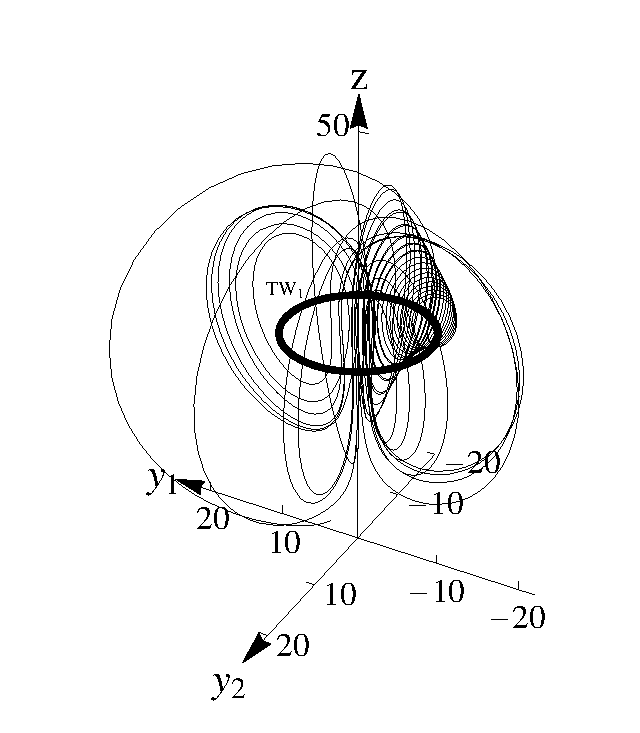
\includegraphics[width=0.45\textwidth]{Fullspace}%
(b)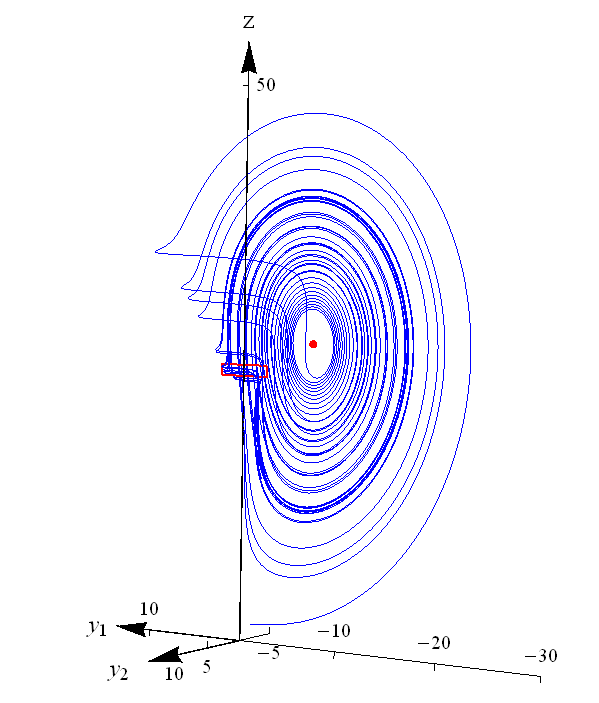
\includegraphics[width=0.38\textwidth]{RedTrajNoPlane1}%
 \end{center}
 \caption{\label{fig:Fullspace}
(color online).
(a) \CLe\ \refeq{eq:CLeR} exhibit a strange attractor for parameter
values \refeq{SiminosPrmts}, here projected on the $\{y_1,y_2,z\}$ axes.
(thin line/blue) A segment of generic finite time trajectory.
(thick line/red)
$\REQV{}{1}$, the only \reqv.
%
% Former {CLEreduced} \label{fig:RedTrajNoPlane1}
(b) The same strange attractor plotted in the symmetry-\reducedsp\
% with initial point
%$(x_1, x_2, y_1, y_2, z) = (1, 2, 3, 1, 2)$
in the slice \refeq{PCsectQ0}, defined by the $\sliceTan{}=(1,0,0,0,0)$.
In the \reducedsp\ \reqv\ $\REQV{}{1}$ is reduced to \eqv\ $\EQV{1}$.
Note, however, the semicircular jumps in the reduced flow. These are
explained and computed in \refsect{sec:singul}. For a blow-up of the jump
indicted by the small rectangle (red), see \reffig{fig:singpass}.
 }%
 \end{figure}

We shall illustrate symmetry reduction by applying it to the
5-dimensional \cLe\rf{GibMcCLE82}
\bea
	\dot{x}_1 &=& -\sigma x_1 + \sigma y_1
\,,\qquad\qquad\qquad
	\dot{x}_2 \,=\, -\sigma x_2 + \sigma y_2
\continue
	\dot{y}_1 &=& (r_1-z)\, x_1  - ~y_1 - e y_2
\,,\qquad\;
	\dot{y}_2 \,=\, (r_1-z)\, x_2 + e y_1 - ~y_2
\continue
	\dot{z}~ &=& -b z + x_1 y_1 + x_2 y_2
\,.
\label{eq:CLeR}
\eea
In all numerical calculations that follow we shall set the
parameters to \refref{SiCvi10} values,
\beq
r_1=28,\; b={8}/{3},\;
\sigma=10,\quad \mbox{and}  \quad e={1}/{10}
\,,
\ee{SiminosPrmts}
for which the flow exhibits a strange attractor,
\reffig{fig:Fullspace}\,(a).
\CLe\ are a simple example of a dynamical system
with a continuous (but no discrete) symmetry.
They are equivariant under \SOn{2} rotations by
\beq
\LieEl(\gSpace)
    \,=\,
\exp{({\gSpace} \cdot \Lg)}
	\,=\,
  \left(\barr{ccccc}
  \cos \gSpace  & \sin \gSpace  & 0 & 0 & 0 \\
 -\sin \gSpace  & \cos \gSpace  & 0 & 0 & 0 \\
 0 & 0 &  \cos \gSpace & \sin \gSpace   & 0 \\
 0 & 0 & -\sin \gSpace & \cos \gSpace   & 0 \\
 0 & 0 & 0             & 0              & 1
    \earr\right)
\,,\qquad
 \Lg \,=\,   \left(\barr{ccccc}
    0  &  1 & 0  &  0 & 0  \\
   -1  &  0 & 0  &  0 & 0 \\
    0  &  0 & 0  &  1 & 0  \\
    0  &  0 &-1  &  0 & 0 \\
    0  &  0 & 0  &  0 & 0
    \earr\right)
\,.
\ee{CLfRots}
The fixed-point subspace \refeq{dscr:InvPoints} of the $\SOn{2}$ symmetry
group of the \cLe\ is the $z$-axis. The velocity \refeq{eq:CLeR} at a
point on the $z$-axis points only in the $z$-direction and so the
trajectory remains on the $z$-axis for all times.
The group is 1\dmn\ and compact, its
elements parameterized by $\gSpace \mbox{ mod } 2\pi$.
The action of \SOn{2}\ thus decomposes the  \statesp\ into $m=0$
\SOn{2}-invariant subspace ($z$-axis) and  $m=1$ subspace of
multiplicity 2. Locally, at
\statesp\ point $\ssp$, the infinitesimal action of the group is
given by the group tangent field $\groupTan(\ssp) = \Lg \ssp
= (x_2,-x_1,y_2,-y_1,0)$, with the flow induced by
the group action normal to the radial direction in the
$(x_1,x_2)$ and $(y_1,y_2)$ planes, while the $z$-axis is left
invariant.
	\PC{
	explain the \statesp\ is foliated by group and time-evolution
	orbits, the reduction is attained by slicing group orbits
	and \PoincSec s for time-evolution
	}

%
% ****** End of file intro.tex ******
